\subsection[Correction to $dN/dn_{ch}$]{Correction to $\mathbf{dN/dn_{ch}}$}\label{section:star_dNdnch}
In order to express the multiplicity distribution in terms of the number of charged particles $n_{ch}$ instead of the number of selected tracks $n_{sel}$,  the observed $n_{sel}$ distribution was corrected for detector effects after the subtraction of accidental and non-SD backgrounds. The  following procedure based on the Bayesian unfolding~\cite{unfolding:2016mok,unfolding:DAgostini} was used. First, the $n_{sel}$ distribution was corrected for vertex reconstruction effects by applying event-by-event $w_{ev}^{vrt}(n_{vrt}^{global},|\Delta z_0|)$ weights. The number of events in which $n_{ch}$ are produced, $N_{ev}(n_{ch})$, can be associated with the number of events in which $n_{sel}$ are reconstructed, $N_{ev}(n_{sel})$:
\begin{equation}
N_{ev}\left(n_{ch}\right)=N_{ev}\left(n_{sel}\right)\cdot P\left(n_{ch}|n_{sel}\right)
\end{equation}
where $P(n_{ch}|n_{sel})$ is the  probability of $n_{ch}$ under condition of $n_{sel}$.


When  there are several possible $n_{sel}$ the number of events in which $n_{ch}$ are produced is given by:
\begin{equation}
\begin{array}{ccccc}
N_{ev}(n_{ch})&=&&\sum_{n_{sel}\geq0}P(n_{ch}|n_{sel})\cdot N_{ev}(n_{sel})\\
&=&\frac{1}{\epsilon^{m}(n_{ch})\epsilon^{r}(n_{ch})}&\sum_{n_{sel}\geq2}P(n_{ch}|n_{sel})\cdot N_{ev}(n_{sel})
\end{array}
\end{equation}
where:
\begin{description}
	\item $\epsilon^{m}(n_{ch})$ is a factor, which recovers events that are lost due to TPC track reconstuction and  TOF matching inefficiencies, i.e. those with $n_{ch}\geq2$ but $n_{sel}<2$,
	\item $\epsilon^{r}(n_{ch})$ is a factor, which recovers  events which are lost due to fake tracks, i.e. those with $n_{ch}\leq 8$ but $n_{sel}> 8$.
\end{description}
Figure~\ref{fig:correctionSTAR} shows $\epsilon^{m}(n_{ch})$ and $\epsilon^{r}(n_{ch})$ in three ranges of $\xi$. Both corrections were derived from MC. The former varies from about $25\%$ for $n_{ch}=2$ to $95\%$ for $n_{ch}=8$, the latter is significantly smaller and varies up to $2\%$ for $n_{ch}=8$.


\begin{figure}[h!]
	\centering
	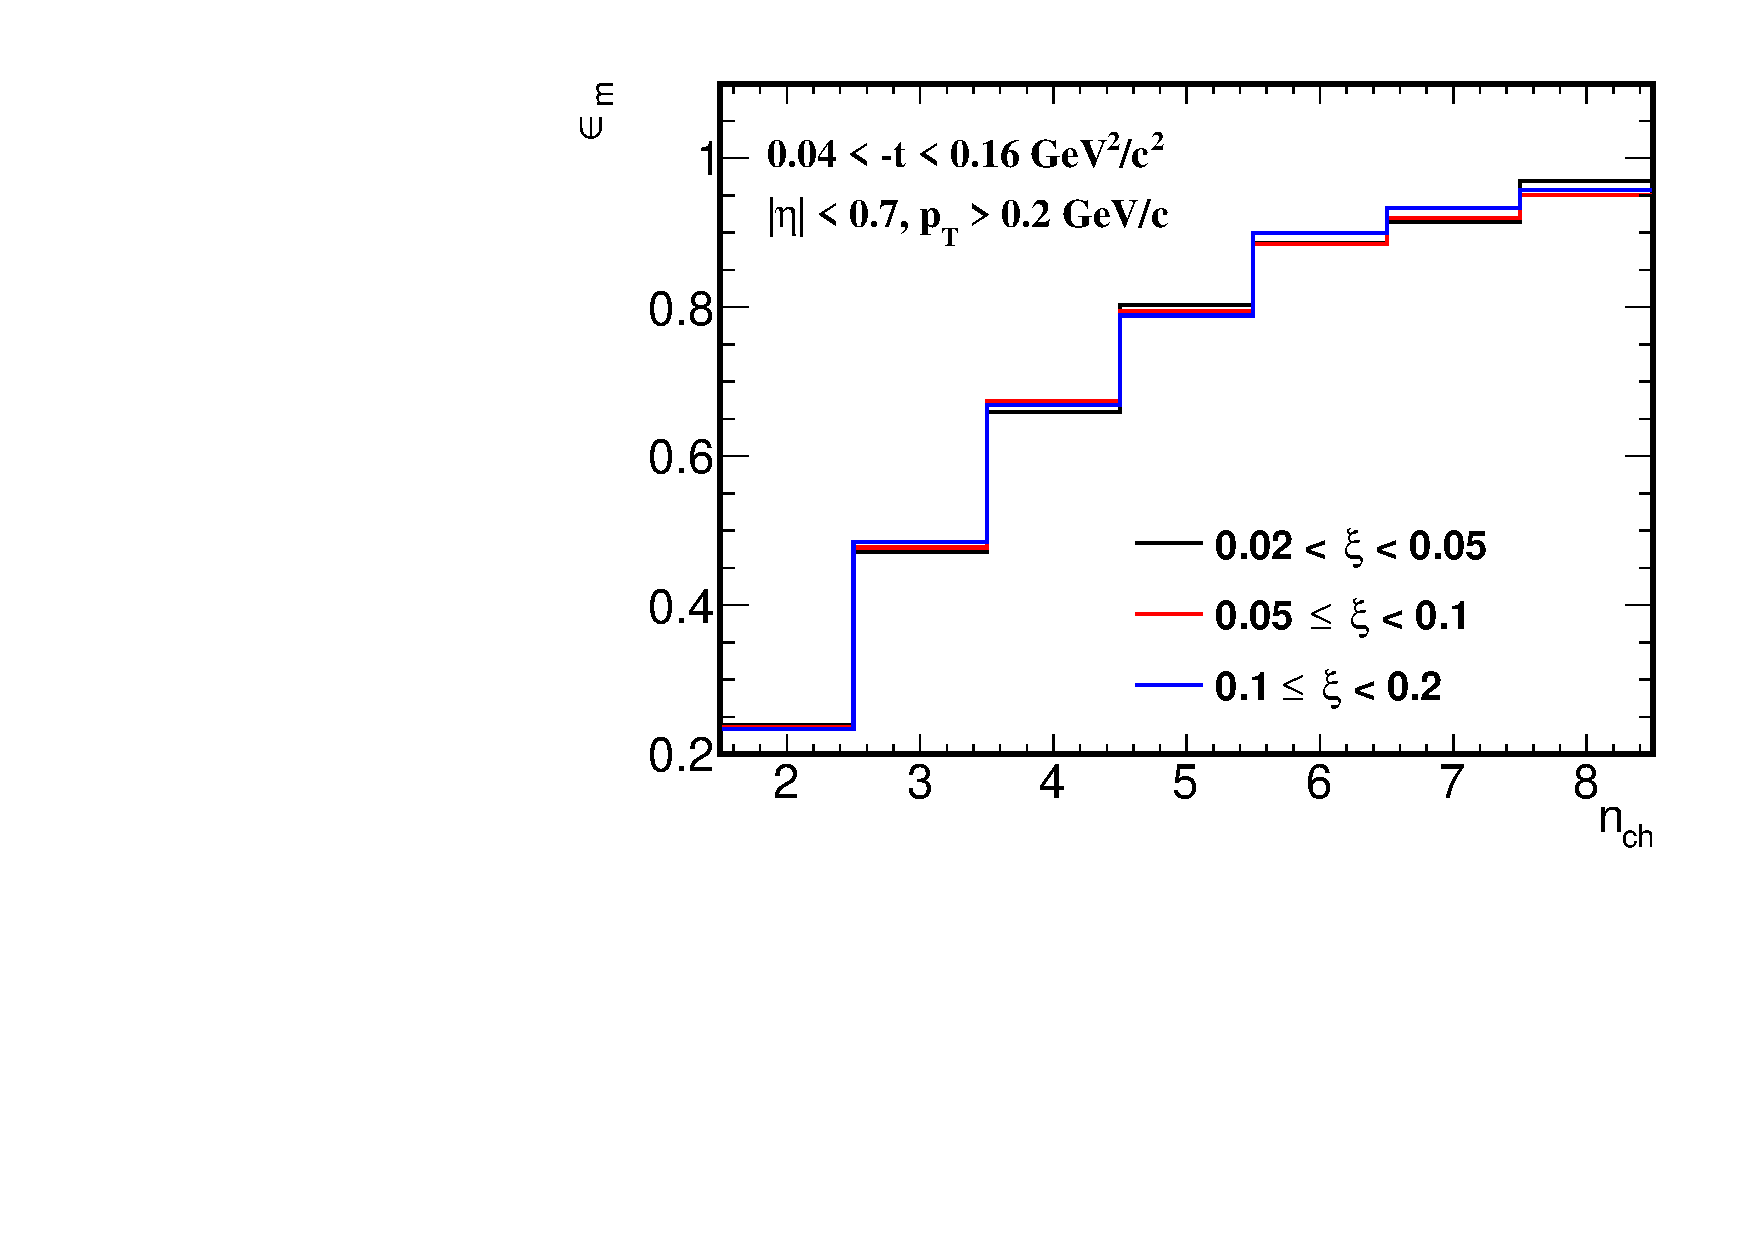
\includegraphics[width=0.49\textwidth,page=1]{chapters/chrgSTAR/img/unfolding/correction_0.pdf}
	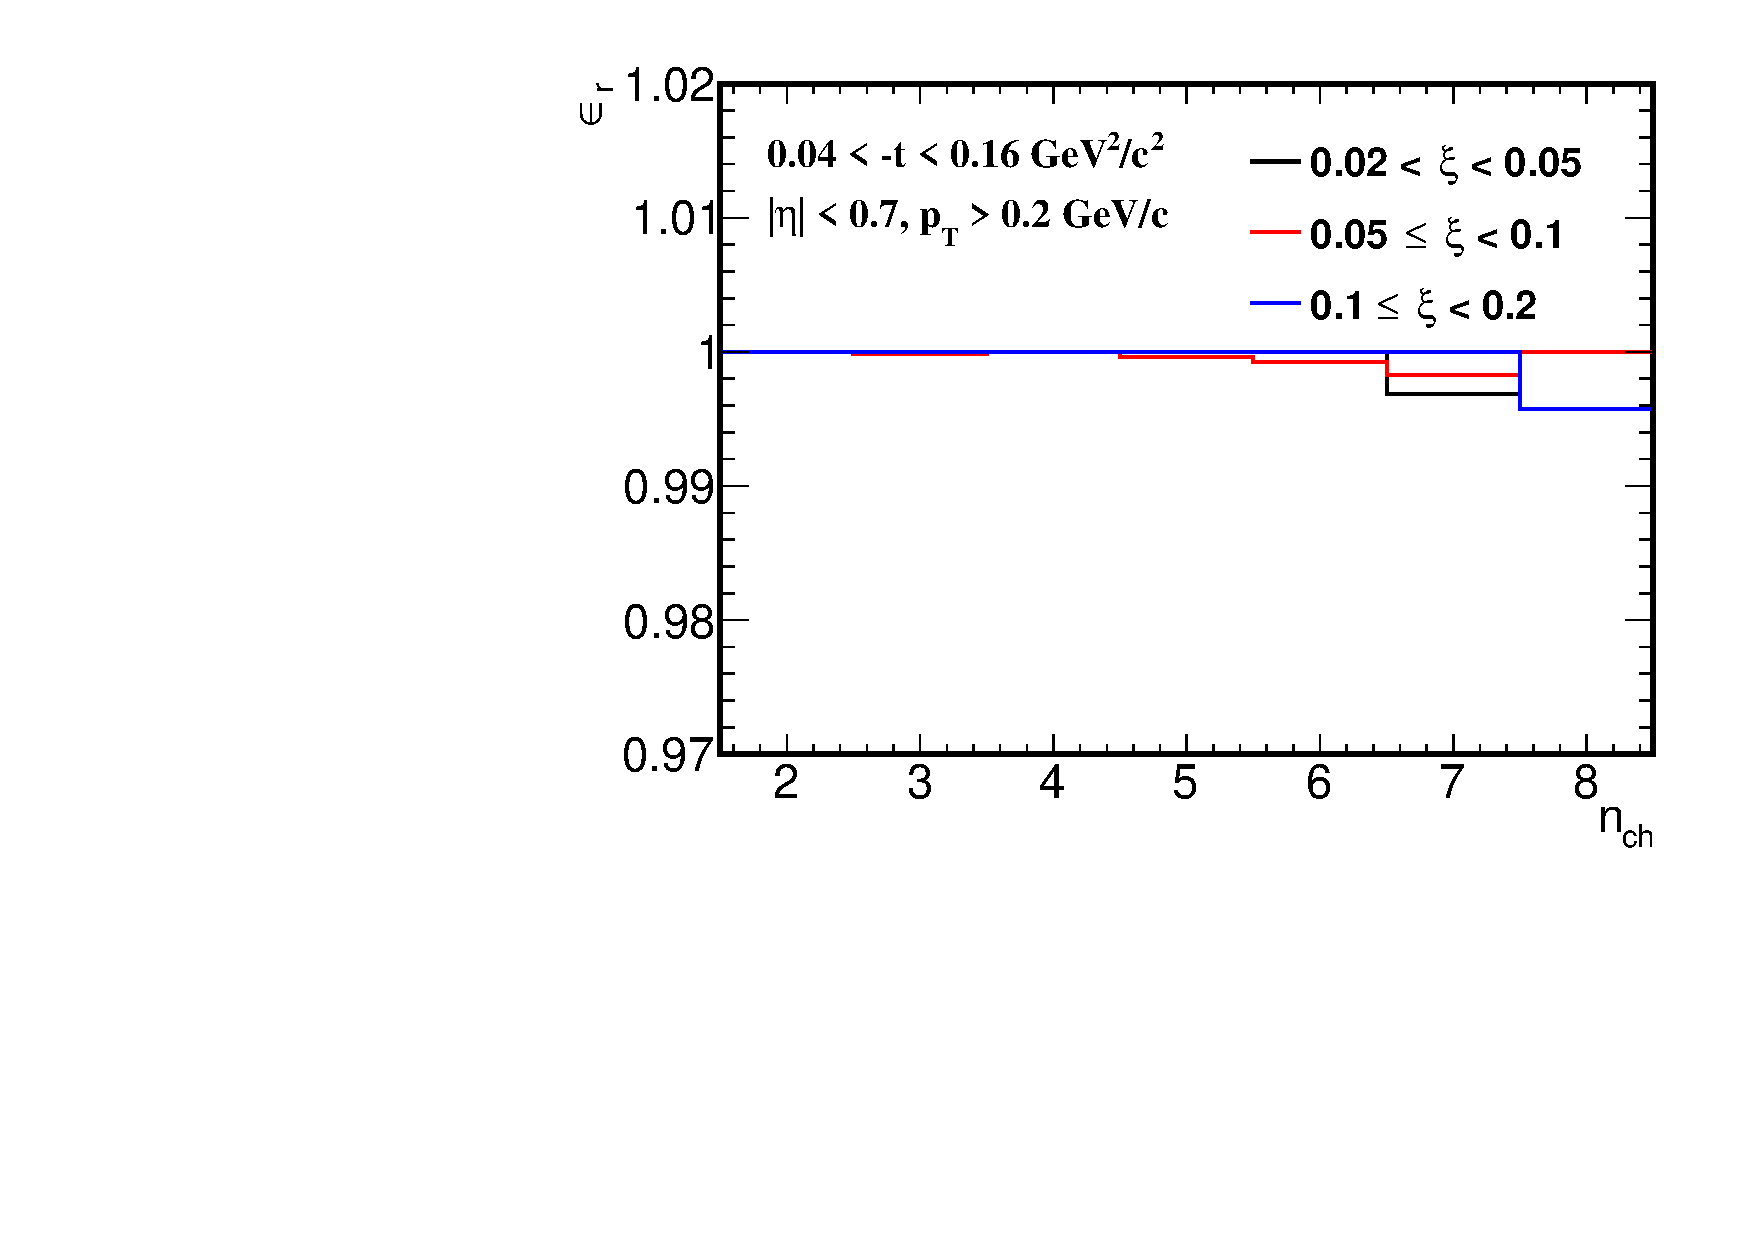
\includegraphics[width=0.49\textwidth,page=1]{chapters/chrgSTAR/img/unfolding/correction_1.pdf}
	\caption[$\epsilon^{m}(n_{ch})$ and $\epsilon^{r}(n_{ch})$ in three ranges of $\xi$]{$\epsilon^{m}(n_{ch})$ (left)  and $\epsilon^{r}(n_{ch})$ (right) calculated separately in three ranges of $\xi$.}
	\label{fig:correctionSTAR}
\end{figure}

The unknown term $P(n_{ch}|n_{sel})$ can be derived through Bayes theorem, which is stated mathematically in terms of charged particle and charged track multiplicities as the following equation:
\begin{equation}
P\left(n_{ch}\right)\cdot P\left(n_{sel}|n_{ch}\right) = P\left(n_{ch}|n_{sel}\right)\cdot P\left(n_{sel}\right)
\end{equation}
where:
\begin{description}
	\item $P(n_{sel})$ and $P(n_{ch})$ are probabilities of observing $n_{sel}$ and $n_{ch}$ independently,
	\item $P(n_{ch}|n_{sel})$ and $P(n_{sel}|n_{ch})$ are conditional probabilities.
\end{description}
 
 The main idea behind these procedure is that the unfolding  is done iteratively to improve the estimate of $P(n_{ch}|n_{sel})$:
\begin{itemize}
	\item First iteration: \\
	\begin{eqnarray}
	P(n_{ch}|n_{sel}) = P = P(n_{sel}|n_{ch})\frac{P^{MC}(n_{ch})}{P^{MC}(n_{sel})}
	\end{eqnarray}
	\begin{equation}
	N_{ev}(n_{ch})=\frac{1}{\epsilon^{m}(n_{ch})\epsilon^{r}(n_{ch})}\sum_{n_{sel}\geq2}N_{ev}(n_{sel})\cdot P
	\end{equation}
	where $P(n_{sel}|n_{ch})$, $P^{MC}(n_{ch})$ and $P^{MC}(n_{sel})$ are obtained from MC. $P(n_{sel}|n_{ch})$ is the same for each iteration.
	
	\item Next iterations $i+1$:
	\begin{equation}
	P^{i+1}=P(n_{sel}|n_{ch})\frac{P^{i}(n_{ch})}{P(n_{sel})}
	\end{equation}
	\begin{equation}
	N_{ev}^{i+1}(n_{ch})=\frac{1}{\epsilon^{m}(n_{ch})\epsilon^{r}(n_{ch})}\sum_{n_{sel}\geq2}N_{ev}(n_{sel})\cdot P^{i+1}
	\end{equation}
	where normalized $N_{ev}^i(n_{ch})$, calculated in the previous iteration, and $N_{ev}(n_{sel})$, taken from data, serve as probability distributions $P^{i}(n_{ch})$ and $P(n_{sel})$.
\end{itemize}

The  unfolding matrices $P(n_{ch}|n_{sel})$  for each $\xi$ region, shown in Fig.~\ref{fig:responseSTAR}, were obtained from MC and used in the first iteration of the above procedure. 

\captionsetup{format=plain,indention=0pt,justification=justified}
\begin{figure}[h!]
	\centering
	\begin{subfigure}{.49\textwidth}
		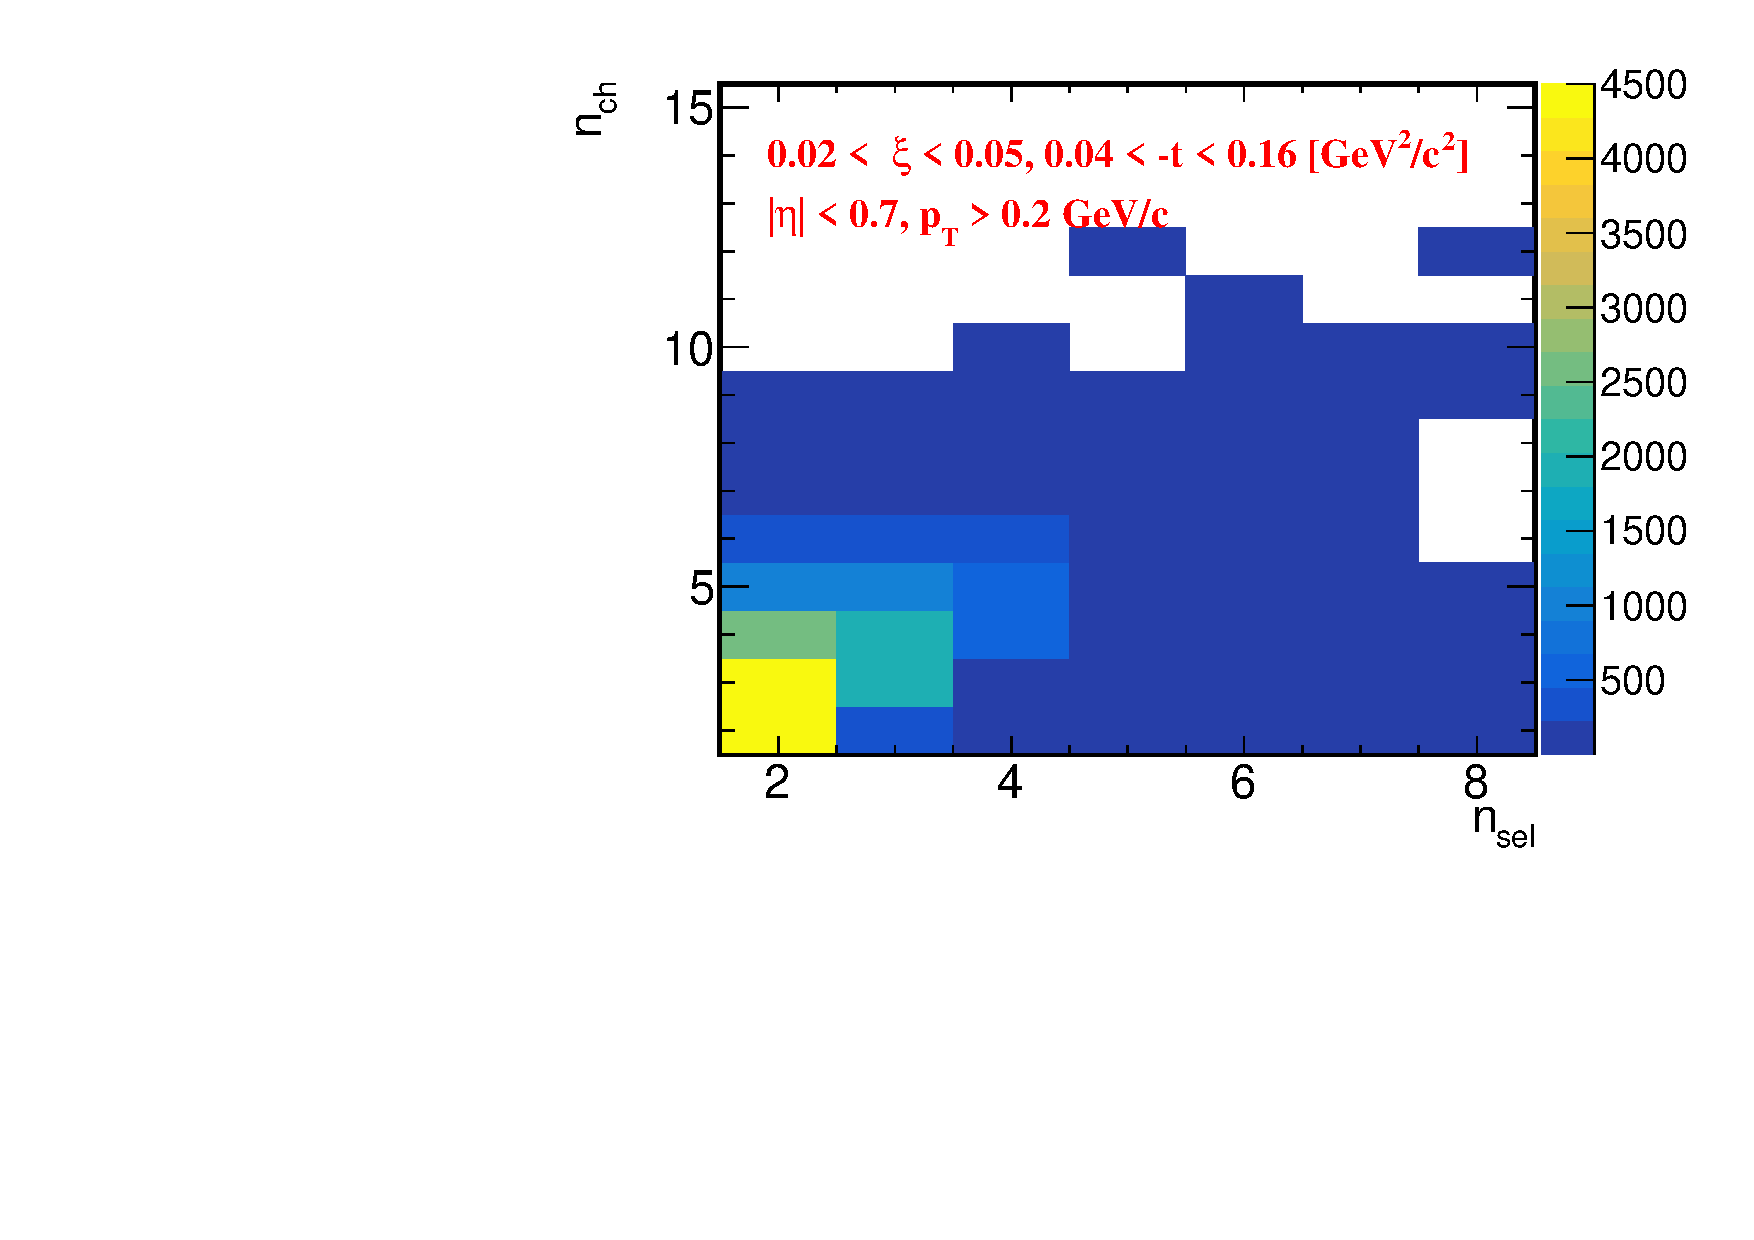
\includegraphics[width=\textwidth,page=1]{chapters/chrgSTAR/img/unfolding/matrix_0.pdf}
	\end{subfigure}
	\begin{subfigure}{.49\textwidth}
		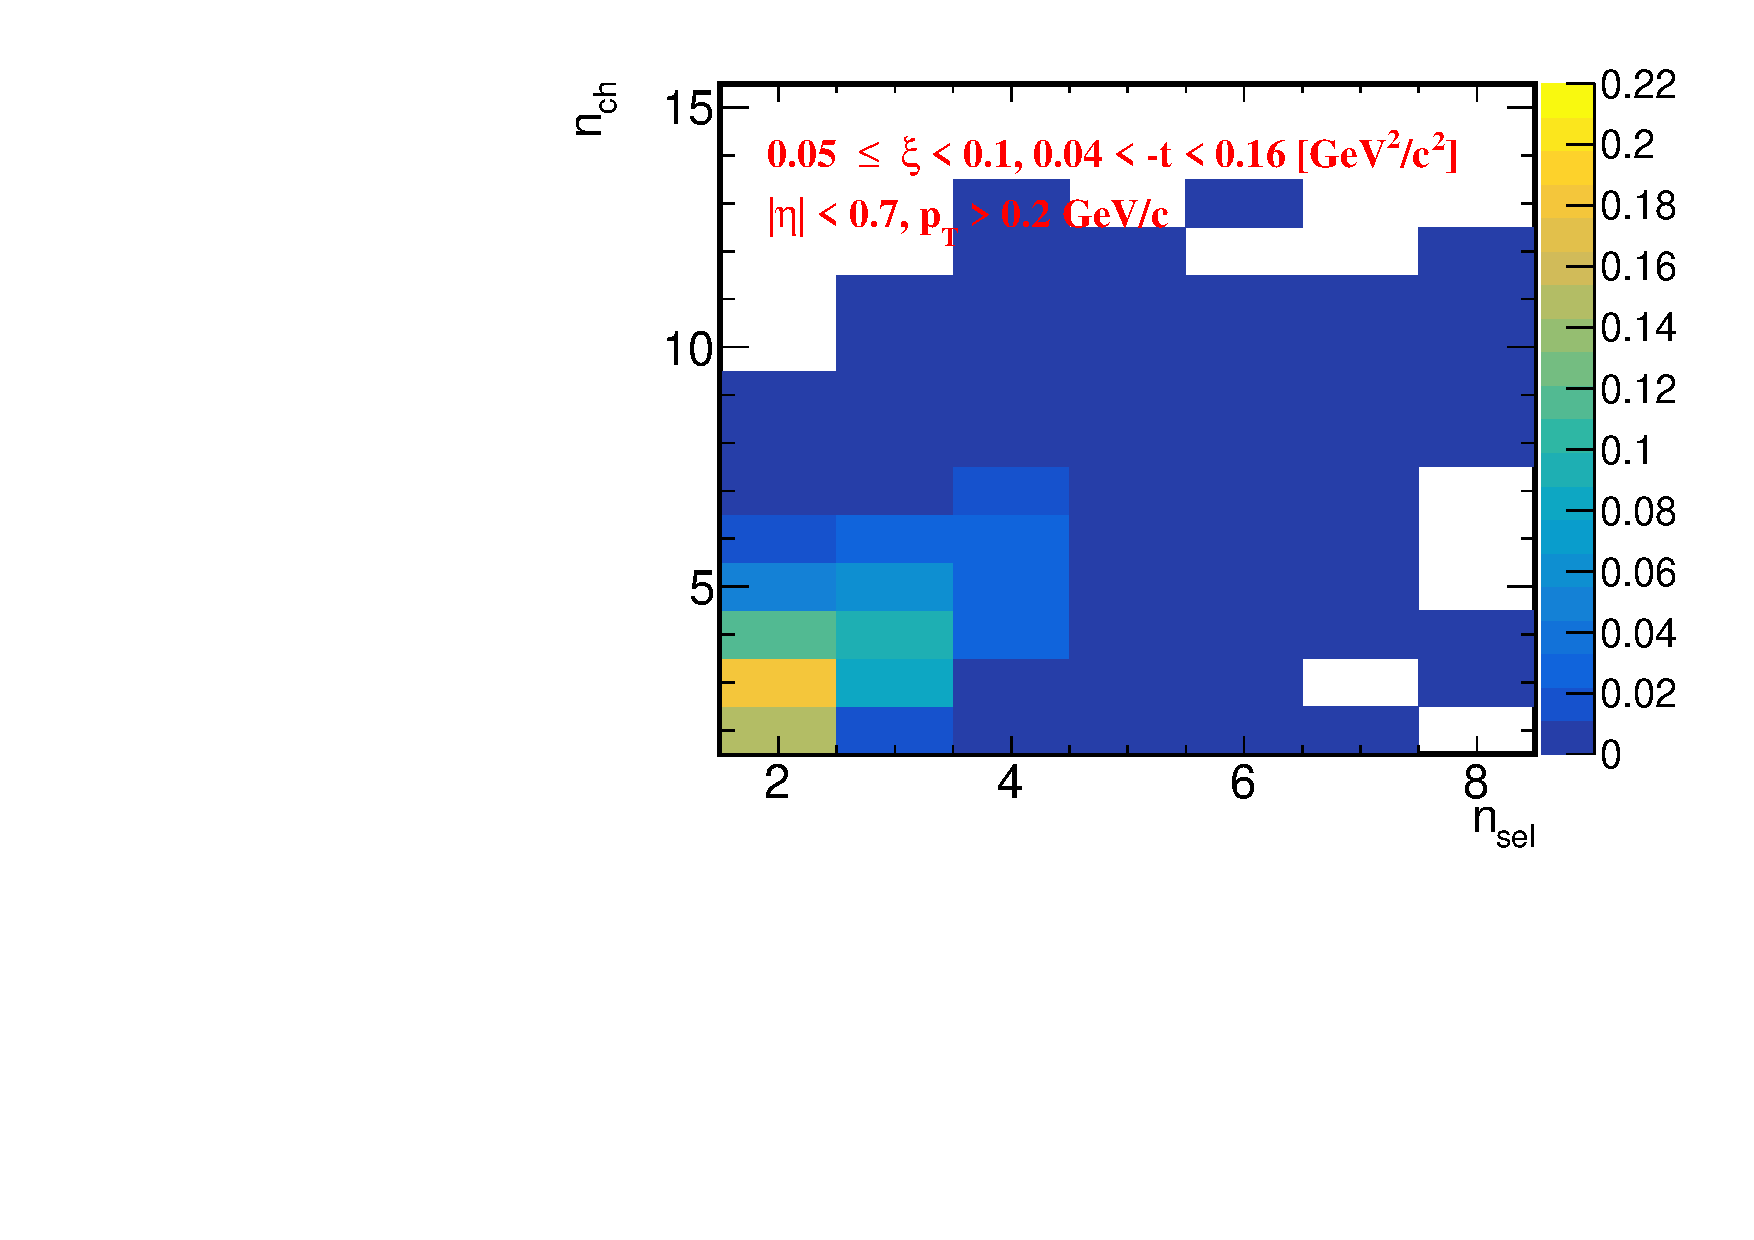
\includegraphics[width=\textwidth,page=1]{chapters/chrgSTAR/img/unfolding/matrix_1.pdf}
	\end{subfigure}
	\begin{subfigure}{.49\textwidth}
		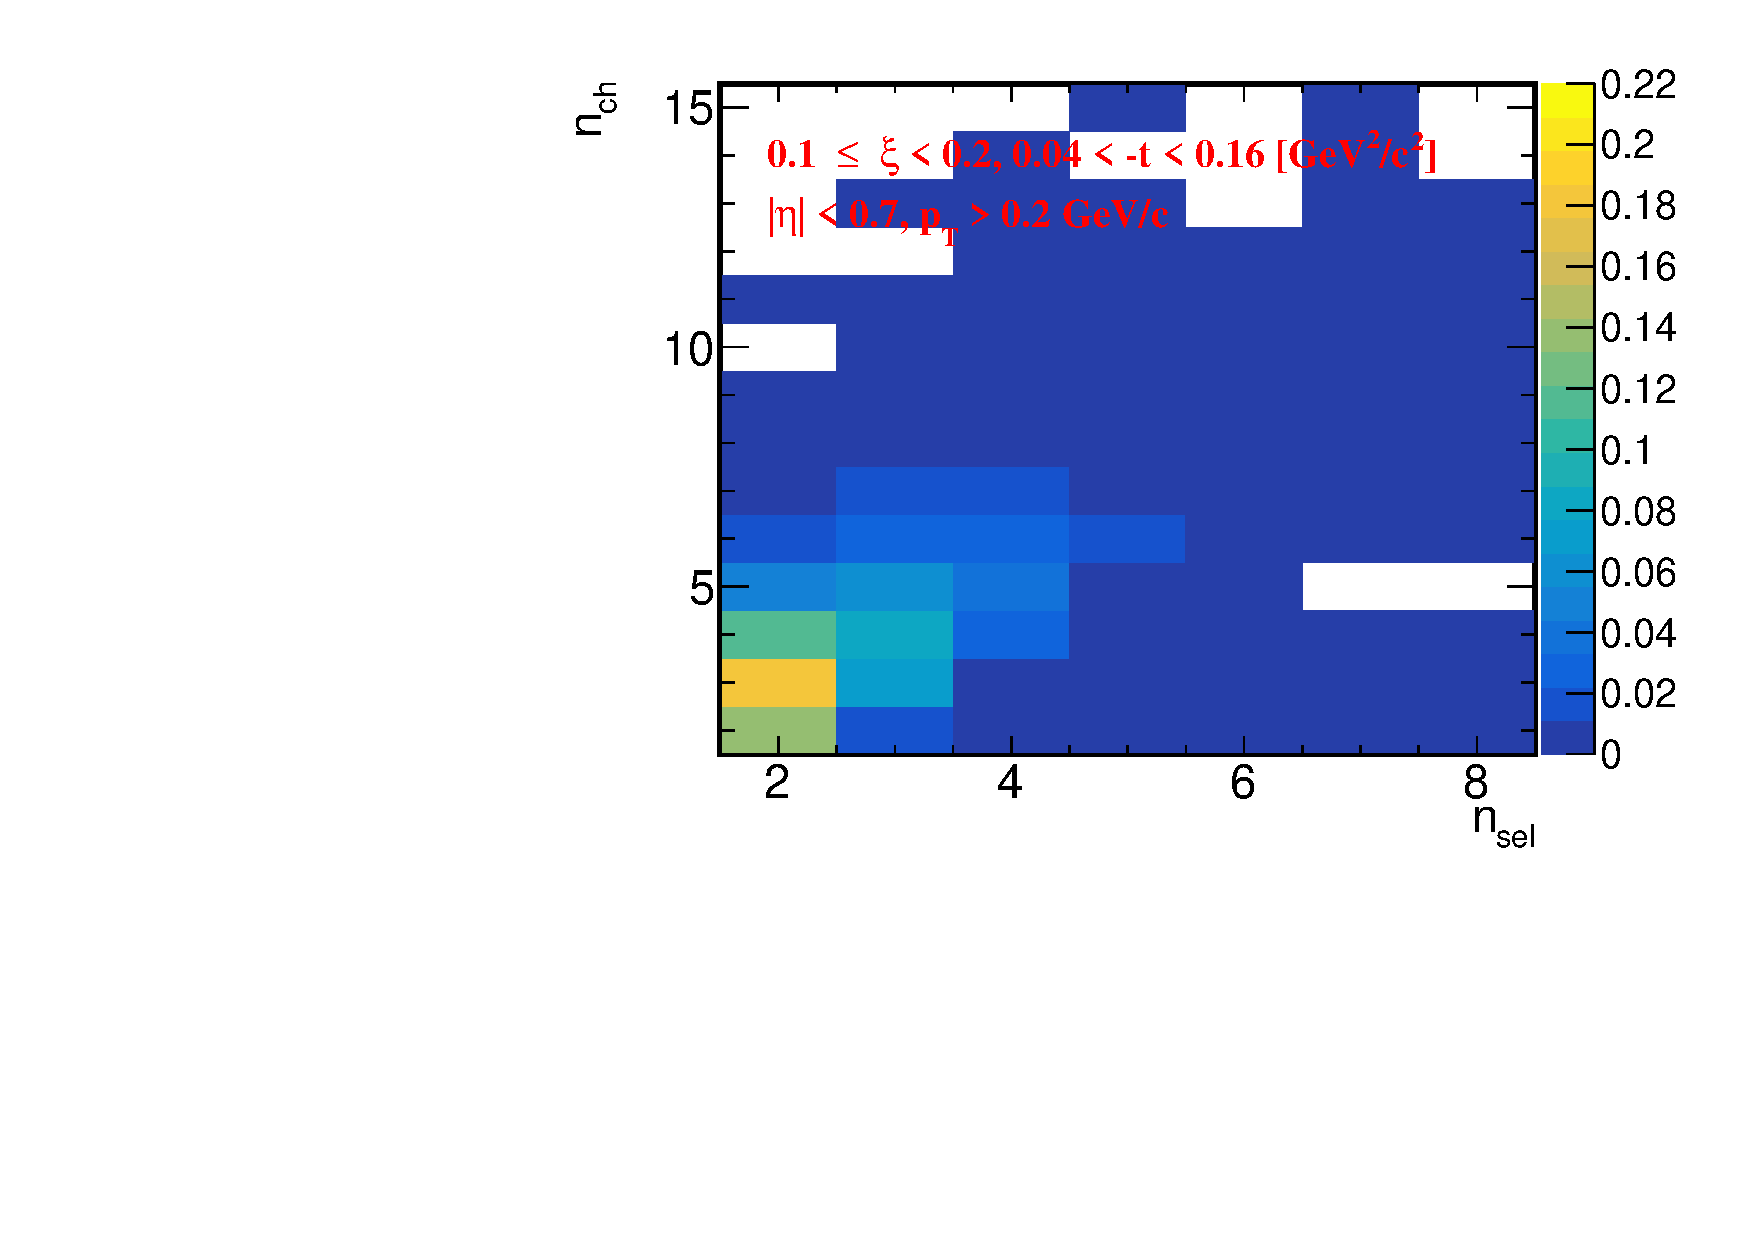
\includegraphics[width=\textwidth,page=1]{chapters/chrgSTAR/img/unfolding/matrix_2.pdf}
	\end{subfigure}
	\begin{minipage}{.49\textwidth}
		\caption{The unfolding matrices calculated  from MC for three ranges of $\xi$ separately.}
		\label{fig:responseSTAR}
	\end{minipage}
\end{figure}
\captionsetup{format=default,indention=0pt,justification=justified}

After the unfolding procedure, the  obtained distribution $dN/dn_{ch}$
was corrected for BBC-small efficiency, through $w_{BBC}(n_{ch})$ weights, and migrations of events between $\xi$ ranges, through $f_{\xi}(n_{ch})$ weights. Since the unfolding matrices contain track reconstruction efficiencies, non-primary track backgrounds, migrations of tracks into and out of the fiducial region, the weight $w_{trk}\left(p_T,\eta,V_{z}\right)$ was not used.

Finally, the $dN/dn_{ch}$ distribution was normalized to total number of events, $N_{ev}=N$, which was calculated as the integral of the unfolded $N_{ev}(n_{ch})$ distribution.



\FloatBarrier